%---=---==---===---====---=====---======---=====---====---===---==---=---%
%-                            SYSTEM TESTING                            -%
%---=---==---===---====---=====---======---=====---====---===---==---=---%

\chapter{Evaluation}\label{chap:evaluation}

Now that everything is implemented, an evaluation of the work is to be completed. This evaluation includes testing, discussions into objectives, literature and requirements, as well a summary for future work.

\section{Testing}

Testing in this project was not able to be extensive due to the large scope covered in research, design and implementation, as well as the limited time available. However, tests that were completed include unit tests and walk-through tests, which follow.

\subsection{Unit Tests}\label{unit}

Unit tests were written for ensuring that the view model for the tower builder application worked as intended, the code for this can be found in \cref{code:unittests}, these unit tests covered two main functions responsible for the addition of blocks to the tower.

Focusing on the \textit{addBlocksTest} class, there are 5 tests and a setup function, which creates the environment with which to test. Further, tests were created logically from the set of possible additions to the tower; no blocks, full row, single block, half full row, and overfull row. Each test includes an assertion which validates the number of blocks on the top row of the tower, for instance, adding 4 blocks to a tower that has a maximum row size of 3, would result in 3 blocks on the first row, and 1 on the top. These tests are necessary because they confirm the functionality of the system, and also serve as an aid when updating or improving the methods.

\begin{figure}[ht]
\hspace*{\fill}
\begin{subfigure}{0.3\textwidth}
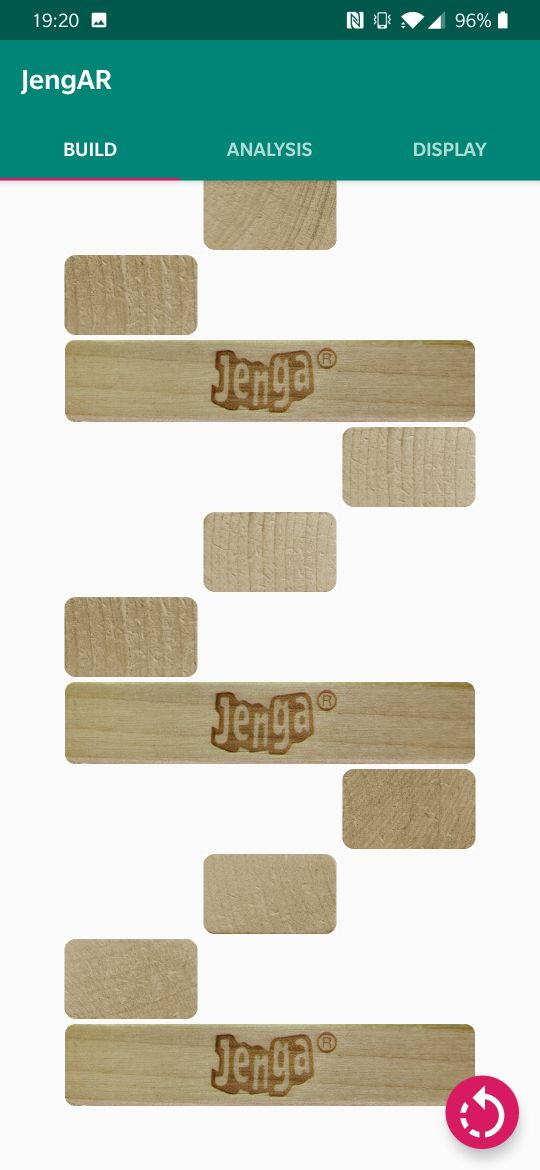
\includegraphics[width=\linewidth]{images/evaluation/uibug.jpg}
\caption{New row bug} \label{fig:uibug1}
\end{subfigure}
\hspace*{\fill}
\begin{subfigure}{0.3\textwidth}
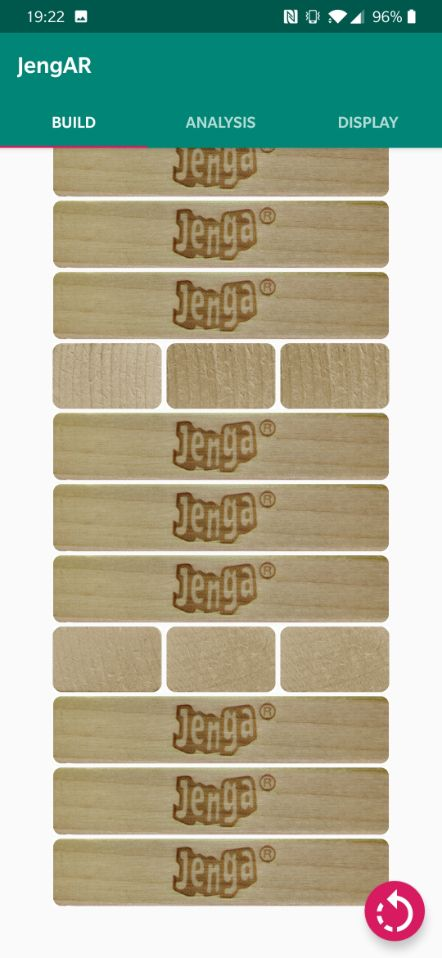
\includegraphics[width=\linewidth]{images/evaluation/uibug2.jpg}
\caption{Side block bug} \label{fig:uibug2}
\end{subfigure}
\hspace*{\fill}
\begin{subfigure}{0.3\textwidth}
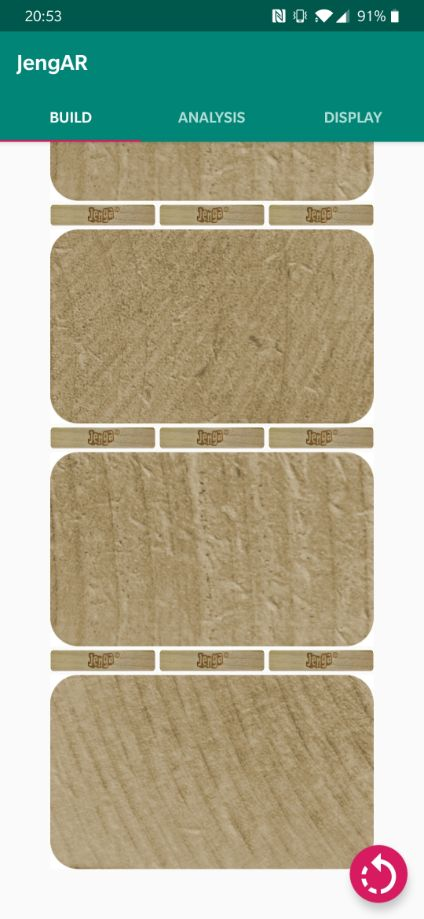
\includegraphics[width=\linewidth]{images/evaluation/uibug3.jpg}
\caption{Size bug} \label{fig:uibug3}
\end{subfigure}
\hspace*{\fill}
\caption{Tower Builder Bugs}
\label{fig:uibugs}
\end{figure}

A few game breaking bugs were found during the development of the tower builder application, shown in \cref{fig:uibugs}. The unit tests written for the view model aided in the solution to these bugs because they were able to validate the soundness of the logic behind the application. In the case of the new row bug, the unit tests failed, determining that the interface was not the point of failure, after fixes were made to the code logic, the bug was solved. Furthermore, the tests were run when the side block bug and size bugs were identified, and it was determined that the code base was functional, meaning that the of the bugs were isolated to the tower drawing class, and were later fixed.

While unit tests are clearly beneficial, it takes a substantial amount of time to obtain full code coverage. Also, although automated interface testing is possible, it was not completed in this project due to time constraints, instead, manual visual feedback was necessary.

\subsection{Detection/Visualisation}\label{det}

Both the detection and visualisation stages same code base, and utilise the same layout, for this reason, it is sufficient to group them up for testing. As can be seen in the video demonstration (\cref{fig:demoqr}), both these stages have issues detecting all markers currently in a frame; while this is not necessary, it is visually displeasing to see markers without the expected augmentation. To fix this, the camera parameters for marker detection could be changed, but this would require to be set up for every different environment, and thus would need to be variable and added to the settings for each user to modify to work with their needs.

\subsection{Analysis}\label{blockapproximation}

Moving forward, the analysis stage was tested thoroughly, examples of this can be found in \cref{chap:results}. A critical issue that was identified in this testing was that blocks would occasionally be generated in the wrong place, this is due to inaccuracies in either: detection and pose estimation of markers, marker localisation and mapping, or approximation of centre point and rotation of blocks.

However, inaccurate block generation was only an issue in certain cases, for instance, when mapping a large number of blocks, i.e. all 54. It was determined that the cause of the error was in the detection stage, and occurred when a large number of markers were shown in a single frame. With there being a large number of markers, it seems that errors are increased in pose estimation. To solve this problem, multiple images per face need to be taken, and so the implementation should be changed to accommodate for this.

On occasion, the reconstruction would be accurate, but then the tower would fall over before any blocks were removed. This is due to some of the blocks overlapping, thus generating large amounts of force inside the tower, causing the blocks to be pushed outwards. The fact that this issue did not occur in every test suggests that again it is a problem with the detection stage, with blocks being detected in slightly the wrong places. Again, this can be solved by holding the camera closer to the tower, thus detecting fewer markers per frame.

\begin{figure}[ht]
    \centering
    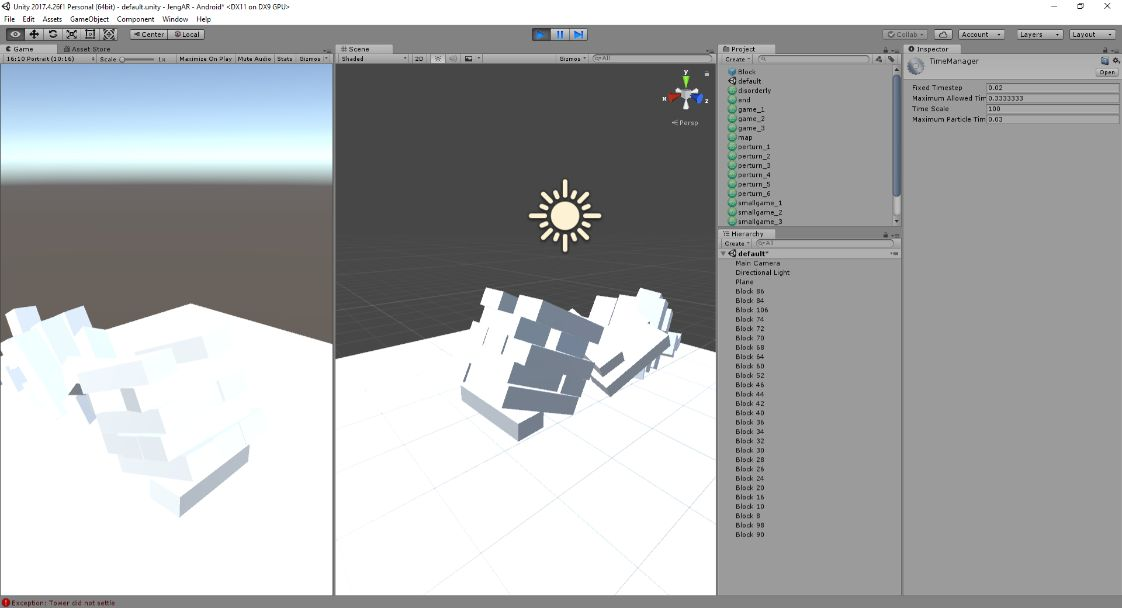
\includegraphics[width=.7\linewidth]{images/testing/smallgame2.jpg}
    \caption{A reconstruction that toppled over before analysis could begin}
    \label{fig:unsettled}
\end{figure}



Moreover, when a virtual tower was reconstructed successfully, the analysis was accurate; blocks marked red were clearly difficult to remove, and green blocks were clearly easy to remove. Although layers near to the top of the tower are out of bounds during the game, due to them being easier to remove, it is still worthwhile to show their removal feasibility to the user for completeness.

\section{Attaining Objectives}

With testing complete, the evaluation moves on to the objectives set at the beginning of the project. This short section shows how all objectives were attained by the end of the time frame of the project.

\hyperref[obj:detect]{Objective 1} was achieved through the use of square planar markers and the ArUco library. This detection method is robust to rotational and translational differences in blocks, and can, therefore, be used in any real-world scenario, unlike competing methods.

Also, \hyperref[obj:analysis]{Objective 2} was reached through the use of the MarkerMapper application, which was able to localise and map the detected markers. The marker map gained was then used to reconstruct the tower in Unity, which was analysed using a state-of-the-art simulation method.

Finally, \hyperref[obj:display]{Objective 3} was accomplished by using a combination of OpenCV and ArUco. Scores sent from the analysis stage were normalised and converted into colours on a green to red scale, which were then successfully displayed to the user, thus completing the system.

\section{Use of Literature}

The \nameandsecref{chap:background} was a substantial part of this project, this section aims to show how the knowledge gained in the literature and technology review was used to aid in the development of the system.

Firstly, the \nameandsecref{sec:reconstruction} looked into the various methods for reconstruction and determined that the most appropriate category was parts-based, and also found that voxel-based and view-based modelling were not sufficient for use in the project. This meant that the project should build the virtual tower from a library of block objects, which subsequently lead to the creation of a Unity GameObject that was used in the creation of virtual blocks.

Secondly, the review of the previous \jenga{} analysis papers showed the various ways in which towers could be analysed for block removal feasibility; namely, \citet{jengarobot} used a simulation method which was the inspiration for the analysis method used in this paper.

Finally, the research into augmented reality SDKs and libraries (\cref{sec:markerbased}) was beneficial because it gave knowledge about the current state of AR, and also identified that MarkerMapper and UcoSLAM were the most appropriate libraries for use in this project, coincidentally MarkerMapper became a crucial part of the reconstruction stage.

\section{Meeting Requirements}

Now that the objectives have been shown to be met, and the use of literature has been established, naturally this section progresses into the state of requirements, and giving reasons as to why certain requirements were or were not met. As there are a couple dozen requirements set for this project, it was deemed worthwhile to only discuss a subset of them in this section, however, a full list of requirements and their statuses can be found in \nameandsecref{chap:requirements}.

To begin with, \cref{req:towerstate} states that the system could be able to detect when the tower has changed state. This requirement was not met because knowledge of the tower is based on a full set of images around its perimeter, meaning that for the system to know whether the tower has changed state, the user would have to essentially run through the whole detection stage, which is done by the user when they want a new analysis anyway.

Further, \cref{req:inaccuracies} was not met because accounting for inaccuracies in pose estimation would require a significant amount of testing and work, that simply didn't fit into the time frame or scope of the project. However, due to the project being maintainable (\cref{req:maintainable}), future work could be done to solve the inaccuracy problem.

The project does not use multiple analysis techniques, which violates \cref{req:multianalysis}. This was decided because of the many possibilities of tower state, meaning that a rule-based analysis would be inaccurate. However, the simulation method provides a robust analysis which takes around 5 seconds for reasonably sized towers, so using this as the sole way to analyse the tower is dignified.

A final note can be made towards the \cref{sec:req:additional} of requirements, which were added part way through the project. This change in requirements was due to library compilation issues, and subsequently caused a lot more work than was initially required for system completion. This increase of scope reduced the amount of time available to spend on other stages of the project, but it was worth the effort because it formed the basis of communication, and allowed for the separation of complexity between server and client.

\section{Future Work}

The final section in this evaluation chapter opens a discussion into the future progression of the project, after the end of the planned time plan. It begins with extensions and maintenance of the system, then does into commercial potential, and finally shows how the system can be used outside of the game of \jenga{}.

\subsection{Extension}

Extensions to the project are endless, ranging from improving the interface, to adding extra techniques and methods. This section aims to identify the most plausible and worthwhile extensions that should be considered when extending the system. Also, with the project being modular (\cref{req:modular}) the complexity of incorporating the following extensions is decreased, when compared with a project that is not built to be modular.

The first extension that comes to mind is the addition of machine learning (ML) into the analysis stage, this is because, as described in \cref{subsec:machinelearning}, ML would fit well into the system. Doing so would potentially increase the accuracy and also decrease the time taken for analysis.

Furthermore, ARCore (\cref{sec:arcore}) would improve the visualisation stage considerably. Currently, OpenCV is used for the display of scores on blocks by drawing filled rectangles in place, but using ARCore the system would be able to display a full tower in a multitude of ways. Particularly, the model reconstructed in Unity could be used to visualise a virtual tower in such a way that it stands next to the real tower, or even overlay the tower completely; this would allow for a more immersive user experience.

Finally, it seems reasonable to suggest that the variants, conceived in \cref{subsec:variation}, should be included in the next release of the system; due to their increase of gamification and thus ability to keep the attention of the user (\cref{req:attention}). The most favoured of which is the challenges variant, this is because players of the game commonly draw on their tower pieces to add challenges, but this gives rise to a problem; more specifically the permanence of writing on blocks means that users cannot change nor remove the challenges. Using augmented reality to add challenges would solve this problem.

\subsection{Commercial Potential}

As well as the numerous possible extensions, this system proposed by this paper has significant commercial potential. For this project to become commercially viable, it should become self-contained (\cref{req:selfcontained}), this would be possible by fixing the compilation issues with MarkerMapper, or developing a marker mapping solution without use of the library. Given this, the system would be able to be deployed to a standalone Android app, and thus make it more accessible to consumers.

Further, the system requires markers to be affixed to blocks; this is a lengthy task which is off-putting to users. However, there are several companies that offer custom printed labels, which could be used to print off AR markers as stickers, thus providing a simpler way to set up the system and also reducing the time spent doing so.

\subsection{External Applications}

The final section in this evaluation describes the possible applications of the system outside the game of \jenga{}, most notably in structural analysis. An example of a possible structure and its analysis can be seen in \cref{fig:structureanalysis}; it shows that the system, without modification, can properly analyse the integrity of a structure, provided markers can be affixed. The analysis shows that the parts towards the lower end are vital to its integrity, and would cause more damage to the structure if they were removed, than the parts at the top.

\begin{figure}[ht]
    \hspace*{\fill}
    \begin{subfigure}{0.3\textwidth}
    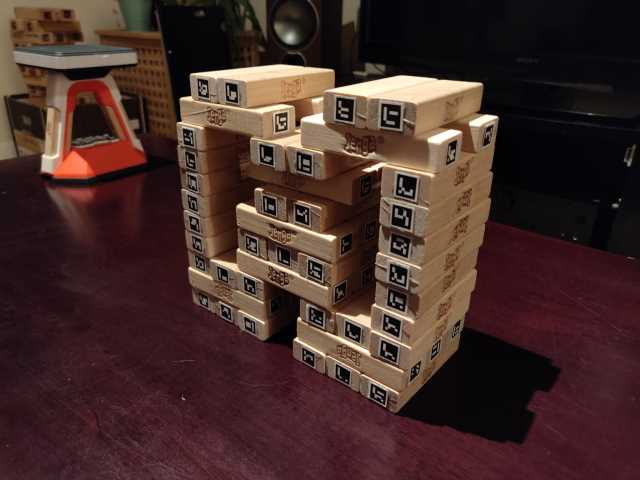
\includegraphics[width=\linewidth]{images/testing/structure-real.jpg}
    \caption{Possible structure} \label{fig:structure}
    \end{subfigure}
    \hspace*{\fill}
    \begin{subfigure}{0.5\textwidth}
    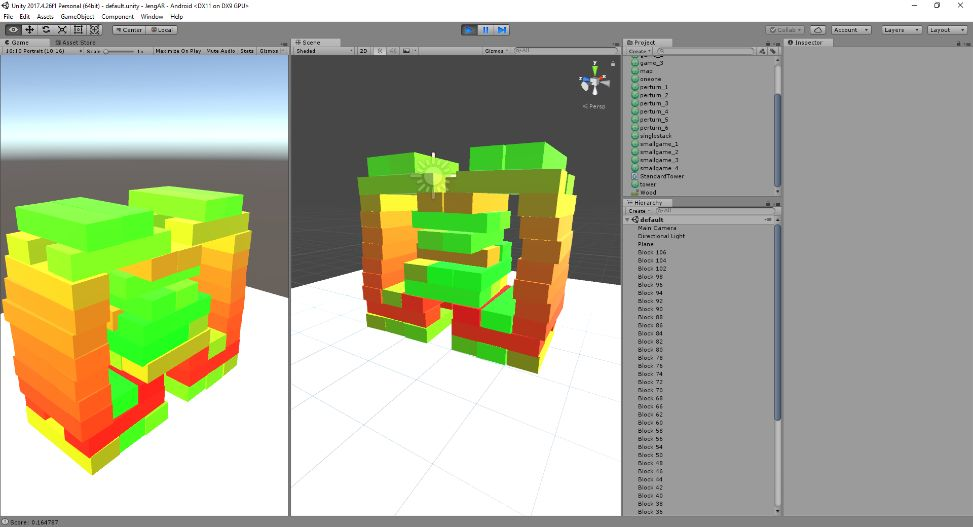
\includegraphics[width=\linewidth]{images/testing/structure.jpg}
    \caption{Structural analysis} \label{fig:structureanalysis}
    \end{subfigure}
    \hspace*{\fill}
\end{figure}
